\model{Reference Types}

\begin{quote}
\begin{minipage}{0.5\linewidth}

\begin{javalst}
int count;
double price;
String name;
Scanner in;

count = 0;
price = 1.99;
name = "Beyonce";
in = new Scanner(System.in);
\end{javalst}

\end{minipage}
\begin{minipage}{0.5\linewidth}

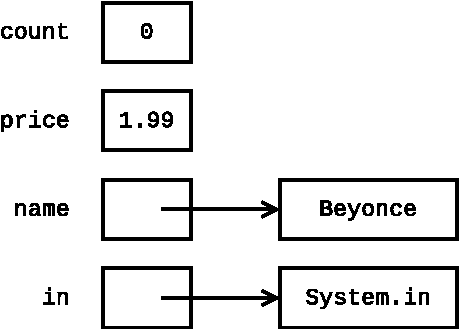
\includegraphics{CS1/reference1.pdf}

\end{minipage}
\end{quote}

Java has eight primitive types (see \ref{CS1/primitive-types}).
All other types of data are called \emph{reference} types, because \textbf{their value is a memory address}.
When drawing memory diagrams, use an arrow to \emph{reference} other memory locations (rather than make up integer values for the actual addresses).


\quest{10 min}


\Q What are the reference types in the example above?

\begin{answer}
\end{answer}


\Q In terms of style, what is the difference between primitive and reference type names?

\begin{answer}
\end{answer}


\Q Variables in Java can use at most eight bytes of memory. Explain why the values for Beyonce and System.in cannot be stored directly in the memory cells for \java{name} and \java{in}.

\begin{answer}
\end{answer}


\Q What is the value of the variable \java{count}? What is the value of the variable \java{price}?

\begin{answer}
\end{answer}


\Q What is the value of the variable \java{name}? What is the value of the variable \java{in}?

\begin{answer}
\end{answer}


\Q \label{assign} Carefully explain what it means to assign one variable to another. For example, what does the statement ~ \java{price = count;}~ do in terms of memory?

\begin{answer}
\end{answer}


\Q Draw a memory diagram for the following code. Make sure your answer is consistent with what you wrote for \ref{assign}.

\begin{javalst}
int width;
float score;
String first;
Scanner input;
String other;

width = 20;
score = 0.94;
first = "Taylor";
input = new Scanner(System.in);
score = width;
other = first;
\end{javalst}
